% answers.tex —— 1993 年·旧科目组·理科 · 参考答案与详细解析片段
% 由 tools/generate_projects.py 依来源总账自 1993/1993_数学真题_旧科目组理_试题.md + 1993/1993_数学真题_旧科目组理_解析正文.md + 1993/1993_数学真题_旧科目组理_答案要点.md 生成，勿手改（改源 MD 后重跑）


\begin{gknotice}
\textbf{解析归属}：固定源 PDF 只有题面，没有答案页。以下推导依据固定题面形成，\textbf{非官方解析}；已由独立解题者在只读题面条件下盲解（29 题），转录另经 400 dpi 逐题复核。第 8、16、28 题的源内疑点在答案要点与本题解析中标注，不以推导结果反改原题。
\end{gknotice}

\begin{answer}
\gksolhead{1}{}

\textbf{题目}：

如果双曲线的实半轴长为 $2$，焦距为 $6$，那么该双曲线的离心率为\mbox{（　　）}。

（A）$\dfrac{\sqrt3}{2}$　　（B）$\dfrac{\sqrt6}{2}$　　（C）$\dfrac32$　　（D）$2$

\Needspace{4\baselineskip}
\textbf{解析}

\gkanswer{答案：C}

\end{answer}
\begin{answer}
\gksolhead{2}{}

\textbf{题目}：

函数 $y=\dfrac{1-\tan^2 2x}{1+\tan^2 2x}$ 的最小正周期是\mbox{（　　）}。

（A）$\dfrac\pi4$　　（B）$\dfrac\pi2$　　（C）$\pi$　　（D）$2\pi$

\Needspace{4\baselineskip}
\textbf{解析}

\gkanswer{答案：B}

\end{answer}
\begin{answer}
\gksolhead{3}{}

\textbf{题目}：

当圆锥的侧面积和底面积的比值是 $\sqrt2$ 时，圆锥的轴截面顶角是\mbox{（　　）}。

（A）$45^\circ$　　（B）$60^\circ$　　（C）$90^\circ$　　（D）$120^\circ$

\Needspace{4\baselineskip}
\textbf{解析}

\gkanswer{答案：C}

\end{answer}
\begin{answer}
\gksolhead{4}{}

\textbf{题目}：

当 $z=-\dfrac{1-i}{\sqrt2}$ 时，$z^{100}+z^{50}+1$ 的值等于\mbox{（　　）}。

（A）$1$　　（B）$-1$　　（C）$i$　　（D）$-i$

\Needspace{4\baselineskip}
\textbf{解析}

\gkanswer{答案：D}

\end{answer}
\begin{answer}
\gksolhead{5}{}

\textbf{题目}：

直线 $bx+ay=ab\ (a<0,\ b<0)$ 的倾斜角是\mbox{（　　）}。

（A）$\arctan\left(-\dfrac ba\right)$　　（B）$\arctan\left(-\dfrac ab\right)$

（C）$\pi-\arctan\dfrac ba$　　（D）$\pi-\arctan\dfrac ab$

\Needspace{4\baselineskip}
\textbf{解析}

\gkanswer{答案：C}

\end{answer}
\begin{answer}
\gksolhead{6}{}

\textbf{题目}：

在直角三角形中两锐角为 $A$ 和 $B$，则 $\sin A\sin B$\mbox{（　　）}。

（A）有最大值 $\dfrac12$ 和最小值 $0$　　（B）有最大值 $\dfrac12$，但无最小值

（C）既无最大值，也无最小值　　（D）有最大值 $1$，但无最小值

\Needspace{4\baselineskip}
\textbf{解析}

\gkanswer{答案：B}

\end{answer}
\begin{answer}
\gksolhead{7}{}

\textbf{题目}：

在各项均为正数的等比数列 $\{a_n\}$ 中，若 $a_5a_6=9$，则 $\log_3a_1+\log_3a_2+\cdots+\log_3a_{10}$ 的值为\mbox{（　　）}。

（A）$12$　　（B）$10$　　（C）$8$　　（D）$2+\log_3 5$

\Needspace{4\baselineskip}
\textbf{解析}

\gkanswer{答案：B}

\end{answer}
\begin{answer}
\gksolhead{8}{}

\textbf{题目}：

$F(x)=\left(1+\dfrac{2}{2^x-1}\right)f(x)\ (x\ne0)$ 是偶函数，且 $f(x)$ 不恒等于零，则 $f(x)$\mbox{（　　）}。

（A）是奇函数　　（B）是偶函数

（C）可能是奇函数也可能是偶函数　　（D）不是奇函数也不是偶函数

\Needspace{4\baselineskip}
\textbf{解析}

在 \(x\ne0\) 上，\(F(x)=f(x)\left(1+\dfrac{2}{2^x-1}\right)\) 为偶函数，而 \(g(x)=1+\dfrac{2}{2^x-1}=\dfrac{2^x+1}{2^x-1}\) 为奇函数且不为零，故 \(f(-x)=-f(x)\)，即 \(f\) 在非零点上为奇函数。题面未给出 \(f(0)\)，按选项取 A；该约定已在答案要点注明。

\gkanswer{答案：A}

\end{answer}
\begin{answer}
\gksolhead{9}{}

\textbf{题目}：

\Needspace{5\baselineskip}
曲线的参数方程为
\nopagebreak[4]
\[
\begin{cases}
x=3t^2+2,\\
y=t^2-1,
\end{cases}\qquad (0\le t\le5),
\]
则曲线是\mbox{（　　）}。

（A）线段　　（B）双曲线的一支　　（C）圆弧　　（D）射线

\Needspace{4\baselineskip}
\textbf{解析}

\gkanswer{答案：A}

\end{answer}
\begin{answer}
\gksolhead{10}{}

\textbf{题目}：

若 $a\text{、}b$ 是任意实数，且 $a>b$，则\mbox{（　　）}。

（A）$a^2>b^2$　　（B）$\dfrac ba<1$

（C）$\lg(a-b)>0$　　（D）$\left(\dfrac12\right)^a<\left(\dfrac12\right)^b$

\Needspace{4\baselineskip}
\textbf{解析}

\gkanswer{答案：D}

\end{answer}
\begin{answer}
\gksolhead{11}{}

\textbf{题目}：

已知集合 $E=\{\theta\mid\cos\theta<\sin\theta,\ 0\le\theta\le2\pi\}$，$F=\{\theta\mid\tan\theta<\sin\theta\}$，那么 $E\cap F$ 为区间\mbox{（　　）}。

（A）$\left(\dfrac\pi2,\pi\right)$　　（B）$\left(\dfrac\pi4,\dfrac{3\pi}4\right)$

（C）$\left(\pi,\dfrac{3\pi}2\right)$　　（D）$\left(\dfrac{3\pi}4,\dfrac{5\pi}4\right)$

\Needspace{4\baselineskip}
\textbf{解析}

\gkanswer{答案：A}

\end{answer}
\begin{answer}
\gksolhead{12}{}

\textbf{题目}：

一动圆与两圆：$x^2+y^2=1$ 和 $x^2+y^2-8x+12=0$ 都外切，则动圆圆心的轨迹为\mbox{（　　）}。

（A）抛物线　　（B）圆　　（C）双曲线的一支　　（D）椭圆

\Needspace{4\baselineskip}
\textbf{解析}

\gkanswer{答案：C}

\end{answer}
\begin{answer}
\gksolhead{13}{}

\textbf{题目}：

若正棱锥的底面边长与侧棱长相等，则该棱锥一定不是\mbox{（　　）}。

（A）三棱锥　　（B）四棱锥　　（C）五棱锥　　（D）六棱锥

\Needspace{4\baselineskip}
\textbf{解析}

\gkanswer{答案：D}

\end{answer}
\begin{answer}
\gksolhead{14}{}

\textbf{题目}：

如果圆柱轴截面的周长 $l$ 为定值，那么圆柱体积的最大值是\mbox{（　　）}。

（A）$\left(\dfrac{l}{6}\right)^3\pi$　　（B）$\left(\dfrac{l}{3}\right)^3\pi$　　（C）$\left(\dfrac{l}{4}\right)^3\pi$　　（D）$\dfrac14\left(\dfrac{l}{4}\right)^3\pi$

\Needspace{4\baselineskip}
\textbf{解析}

\gkanswer{答案：A}

\end{answer}
\begin{answer}
\gksolhead{15}{}

\textbf{题目}：

由 $(\sqrt3x+\sqrt[3]2)^{100}$ 展开所得的 $x$ 的多项式中，系数为有理数的共有\mbox{（　　）}。

（A）$50$ 项　　（B）$17$ 项　　（C）$16$ 项　　（D）$15$ 项

\Needspace{4\baselineskip}
\textbf{解析}

\gkanswer{答案：B}

\end{answer}
\begin{answer}
\gksolhead{16}{}

\textbf{题目}：

设 $a\text{、}b\text{、}c$ 都是正数，且 $3a=4b=6c$，那么\mbox{（　　）}。

（A）$\dfrac1c=\dfrac1a+\dfrac1b$　　（B）$\dfrac2c=\dfrac2a+\dfrac1b$\par\vspace*{3pt}

（C）$\dfrac1c=\dfrac2a+\dfrac2b$　　（D）$\dfrac2c=\dfrac1a+\dfrac2b$

\Needspace{4\baselineskip}
\textbf{解析}

\Needspace{5\baselineskip}
按通行读法 \(3^a=4^b=6^c=k\)，则 \(\dfrac1a=\dfrac{\ln3}{\ln k}\)、\(\dfrac1b=\dfrac{\ln4}{\ln k}\)、\(\dfrac1c=\dfrac{\ln6}{\ln k}\)，于是
\nopagebreak[4]
\[
\dfrac2c=\dfrac{2\ln6}{\ln k}=\dfrac{2\ln3+\ln4}{\ln k}=\dfrac2a+\dfrac1b,
\]
即 (B)。若按字面 \(3a=4b=6c=k\)（\(a=k/3,b=k/4,c=k/6\)）逐项代入，四选项均不成立，故原题应为指数式、上标在转录中丢失；题面照录，答案按指数式并标条件结论。

\gkanswer{答案：B（条件结论：源印 \(3a=4b=6c\) 无上标；按 \(3^a=4^b=6^c\) 得 B）}

\end{answer}
\begin{answer}
\gksolhead{17}{}

\textbf{题目}：

同室四人各写一张贺年卡，先集中起来，然后每人从中拿一张别人送出的贺年卡，则四张贺年卡不同的分配方式有\mbox{（　　）}。

（A）$6$ 种　　（B）$9$ 种　　（C）$11$ 种　　（D）$23$ 种

\Needspace{4\baselineskip}
\textbf{解析}

\gkanswer{答案：B}

\end{answer}
\begin{answer}
\gksolhead{18}{}

\textbf{题目}：

已知异面直线 $a$ 与 $b$ 所成的角为 $50^\circ$，$P$ 为空间上一定点，则过点 $P$ 且与 $a\text{、}b$ 所成的角都是 $30^\circ$ 的直线有且仅有\mbox{（　　）}。

（A）$1$ 条　　（B）$2$ 条　　（C）$3$ 条　　（D）$4$ 条

\Needspace{4\baselineskip}
\textbf{解析}

\gkanswer{答案：B}

\end{answer}
\begin{answer}
\gksolhead{19}{}

\textbf{题目}：

抛物线 $y^2=4x$ 的弦 $AB$ 垂直于 $x$ 轴，若 $AB$ 的长为 $4\sqrt3$，则焦点到 $AB$ 的距离为\underline{\qquad\qquad}。

\Needspace{4\baselineskip}
\textbf{解析}

\gkanswer{答案：\(2\)}

\end{answer}
\begin{answer}
\gksolhead{20}{}

\textbf{题目}：

在半径为 $30\,\mathrm m$ 的圆形广场中央上空，设置一个照明光源，射向地面的光呈圆锥形，且其轴截面顶角为 $120^\circ$。若要光源恰好照亮整个广场，则其高度应为\underline{\qquad\qquad}$\,\mathrm m$（精确到 $0.1\,\mathrm m$）。

\Needspace{4\baselineskip}
\textbf{解析}

\gkanswer{答案：\(10\sqrt3\approx17.3\)}

\end{answer}
\begin{answer}
\gksolhead{21}{}

\textbf{题目}：

在 $50$ 件产品中有 $4$ 件是次品，从中任意抽出 $5$ 件，至少有 $3$ 件是次品的抽法共\underline{\qquad\qquad}种（用数字作答）。

\Needspace{4\baselineskip}
\textbf{解析}

\gkanswer{答案：\(4186\)}

\end{answer}
\begin{answer}
\gksolhead{22}{}

\textbf{题目}：

建造一个容积为 $8\,\mathrm m^3$、深为 $2\,\mathrm m$ 的长方体无盖水池，如果池底和池壁的造价每平方米分别为 $120$ 元和 $80$ 元，那么水池的最低总造价为\underline{\qquad\qquad}元。

\Needspace{4\baselineskip}
\textbf{解析}

\gkanswer{答案：\(1760\) 元}

\end{answer}
\begin{answer}
\gksolhead{23}{}

\textbf{题目}：

设 $f(x)=4^x-2^{x+1}$，则 $f^{-1}(0)=$\underline{\qquad\qquad}。

\Needspace{4\baselineskip}
\textbf{解析}

\gkanswer{答案：\(1\)}

\end{answer}
\begin{answer}
\gksolhead{24}{}

\textbf{题目}：

已知等差数列 $\{a_n\}$ 的公差 $d>0$，首项 $a_1>0$，$S_n=\displaystyle\sum_{i=1}^{n}\dfrac1{a_i a_{i+1}}$，则 $\displaystyle\lim_{n\to\infty}S_n=$\underline{\qquad\qquad}。

\Needspace{4\baselineskip}
\textbf{解析}

\gkanswer{答案：\(\dfrac{1}{a_1d}\)}

\end{answer}
\begin{answer}
\gksolhead{25}{}

\textbf{题目}：

解不等式：$2+\log_{\frac12}(5-x)+\log_2\dfrac1x>0$。

\Needspace{4\baselineskip}
\textbf{解析}

\gkanswer{答案：\((0,1)\cup(4,5)\)}

\end{answer}
\begin{answer}
\gksolhead{26}{}

\textbf{题目}：

如图，$A_1B_1C_1-ABC$ 是直三棱柱，过点 $A_1\text{、}B\text{、}C_1$ 的平面和平面 $ABC$ 的交线记作 $l$。

(1) 判定直线 $A_1C_1$ 和 $l$ 的位置关系，并加以证明；

(2) 若 $A_1A=1$，$AB=4$，$BC=3$，$\angle ABC=90^\circ$，求顶点 $A_1$ 到直线 $l$ 的距离。
\nopagebreak[4]
\begin{center}% f1993_old_science_q26_prism.tex — 1993 年·旧科目组·理科 第 26 题（三棱柱）
%
% 【来源】`.work/phase4-b18/source/1993旧科目组理.pdf`（SHA-256 f4dbb9478d9db142be67604309754f0d0bb5f55be662e5004209cbad60ca0d75），第 1 页；
%   内容流逐路径照录，本地坐标 = 页面坐标 − (1029.610,637.356)，1 单位 = 1 TeX pt。
%   线宽 0.398pt；虚线 [2.989 2.989] 0 d。与文科第 27 题图几何完全一致（纵向平移 232.416pt）。
%
% 标签相对源中心微调：A₁ 左移 1.49pt、B₁ 右上移 (2.5,4.04)pt、C₁ 右上移 (2.2,2.24)pt，避开顶点与边线
% 元素计数：实线 10 段＋虚线 1 段＋6 个标签。
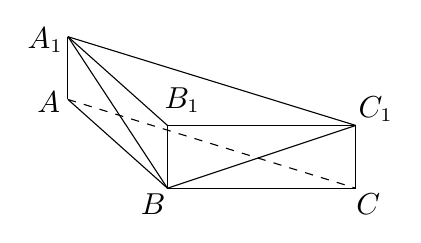
\begin{tikzpicture}[x=1pt, y=1pt,
    every node/.style={inner sep=0pt, font=\fontsize{10.5pt}{12.6pt}\selectfont}]
  \draw[line width=0.398pt] (0.000,32.068) -- (35.968,0.000);
  \draw[line width=0.398pt] (104.005,0.000) -- (35.968,0.000);
  \draw[line width=0.398pt] (0.000,54.747) -- (35.968,22.679);
  \draw[line width=0.398pt] (0.000,54.747) -- (104.005,22.679);
  \draw[line width=0.398pt] (35.968,0.000) -- (35.968,22.679);
  \draw[line width=0.398pt] (0.000,32.068) -- (0.000,54.747);
  \draw[line width=0.398pt] (104.005,22.679) -- (35.968,22.679);
  \draw[line width=0.398pt] (104.005,22.679) -- (35.968,0.000);
  \draw[line width=0.398pt] (0.000,54.747) -- (35.968,0.000);
  \draw[line width=0.398pt] (104.005,22.679) -- (104.005,0.000);
  % 虚线：不可见棱 A₁C
  \draw[line width=0.398pt, dash pattern=on 2.989pt off 2.989pt] (0.000,32.068) -- (104.005,0.000);
  \node[anchor=center] at (-8.200,53.444) {$A_1$};
  \node[anchor=center] at (41.290,31.884) {$B_1$};
  \node[anchor=center] at (111.200,28.584) {$C_1$};
  \node[anchor=center] at (-6.970,31.214) {$A$};
  \node[anchor=center] at (30.770,-5.786) {$B$};
  \node[anchor=center] at (108.560,-5.786) {$C$};
\end{tikzpicture}
%
% 【自验结果】坐标逐点照录内容流；标签取 pdftotext -bbox 中心。
\end{center}
\nopagebreak[4]
\Needspace{4\baselineskip}
\textbf{解析}

\gksubpart{(1)}

设 $B=(0,0,0), A=(4,0,0), C=(0,3,0)$，由直棱柱高1取 $A_1=(4,0,1),C_1=(0,3,1)$。平面 $A_1BC_1$ 内的方向 $\overrightarrow{A_1C_1}=(-4,3,0)$ 平行于底面；它与底面 $ABC$ 的交线 $l$ 因而平行于 $A_1C_1$。

\gksubpart{(2)}

平面法向量可取 $(-3,-4,12)$，平面方程为 $-3x-4y+12z=0$，故底面交线为 $3x+4y=0$。取该线方向 $v=(4,-3,0)$，则 $|v|=5$，点 $A_1$ 至过原点且方向为 $v$ 的直线距离为 $|A_1\times v|/|v|=13/5$。

\gkanswer{答案（1）：\(A_1C_1\parallel l\)}

\gkanswer{答案（2）：\(\dfrac{13}{5}\)}

\end{answer}
\begin{answer}
\gksolhead{27}{}

\textbf{题目}：

在面积为 $1$ 的 $\triangle PMN$ 中，$\tan M=\dfrac12$，$\tan N=-2$，建立适当的坐标系，求出以 $M\text{、}N$ 为焦点且过点 $P$ 的椭圆方程。

\Needspace{4\baselineskip}
\textbf{解析}

\gkanswer{答案：\(\dfrac{x^2}{15/4}+\dfrac{y^2}{3}=1\)}

\end{answer}
\begin{answer}
\gksolhead{28}{}

\textbf{题目}：

设复数 $z=\cos\theta+i\sin\theta\ (0<\theta<\pi)$，$\omega=\dfrac{1-(\overline z)^4}{1+z^4}$，已知 $|\omega|=\dfrac{\sqrt3}{3}$，$\arg\omega=\dfrac\pi2$，求 $\theta$。

\Needspace{4\baselineskip}
\textbf{解析}

\textbf{待核：按当前转录题设无解。} 令 $z=e^{i\theta}$。在原式有定义处，$\omega=\dfrac{1-e^{-4i\theta}}{1+e^{4i\theta}}=i e^{-4i\theta}\tan2\theta$，故 $|\omega|=|\tan2\theta|$。模长条件在 $0<\theta<\pi$ 下只给 $\theta=\pi/12,5\pi/12,7\pi/12,11\pi/12$。逐一代入上式，$\arg\omega$ 分别为 $\pi/6,-\pi/6,\pi/6,-\pi/6$（模 $2\pi$），都不是题设的 $\pi/2$。当前转录条件彼此不相容；须先核原版符号/条件，不能擅自改题以制造答案。

\gkanswer{答案：（条件结论）按题面无解；若分母为 \(1+\overline z^4\)，则 \(\theta=\dfrac{\pi}{12}\) 或 \(\dfrac{7\pi}{12}\)}

\end{answer}
\begin{answer}
\gksolhead{29}{}

\textbf{题目}：

已知关于 $x$ 的实系数二次方程 $x^2+ax+b=0$ 有两个实数根 $\alpha\text{、}\beta$。证明：

(1) 如果 $|\alpha|<2$，$|\beta|<2$，那么 $2|a|<4+b$ 且 $|b|<4$；

(2) 如果 $2|a|<4+b$ 且 $|b|<4$，那么 $|\alpha|<2$，$|\beta|<2$。

\Needspace{4\baselineskip}
\textbf{解析}

\gksubpart{(1)}

记 $p(x)=x^2+ax+b=(x-\alpha)(x-\beta)$。有 $p(2)=(2-\alpha)(2-\beta)=4+2a+b$，$p(-2)=(-2-\alpha)(-2-\beta)=4-2a+b$。

若 $|\alpha|,|\beta|<2$，则 $2-\alpha,2-\beta,-2-\alpha,-2-\beta$ 的成对乘积都为正，故 $p(2)>0,p(-2)>0$，即 $4+b>2|a|$；且 $|b|=|\alpha\beta|<4$。

\gksubpart{(2)}

反之，条件 $2|a|<4+b$ 等价于 $p(2)>0$ 且 $p(-2)>0$；另有 $|\alpha\beta|=|b|<4$。因根为实数，两个端点处多项式均为正，根要么都在 $(-\infty,-2)$、都在 $(-2,2)$，或都在 $(2,\infty)$。若两根都在任一外侧区间，则 $|\alpha\beta|>4$，与 $|b|<4$ 矛盾。因此两根都严格位于 $(-2,2)$。

\gkanswer{答案（1）：见解析（由 \(p(2)>0\)、\(p(-2)>0\) 及 \(|b|<4\) 推得）}

\gkanswer{答案（2）：见解析（由两根分布与 \(|b|<4\) 排除外侧区间）}

\end{answer}